\documentclass[croatian, 12pt]{report}

\usepackage[scaled]{helvet}
\renewcommand\familydefault{\sfdefault} 
\usepackage[T1]{fontenc}

\usepackage[a4paper]{geometry}
\usepackage{pdfpages}
\usepackage{setspace}
\usepackage[utf8]{inputenc}
\usepackage{graphicx}
\usepackage{babel}
\usepackage{hyphsubst}
\usepackage{titlesec}
\usepackage{listings}
\usepackage{svg}
\usepackage[most]{tcolorbox}
\tcbuselibrary{listingsutf8}
\usepackage{inconsolata}
\usepackage{csquotes}
\usepackage[shortlabels]{enumitem}
\usepackage[hidelinks]{hyperref}
\usepackage[backend=biber,style=numeric,url=true,sorting=none]{biblatex}
\usepackage{subfig}
\addbibresource{references.bib}
\bibliography{references.bib}

\titleformat{\chapter}[hang] 
{\normalfont\huge\bfseries}{\thechapter}{1em}{} 

\hypersetup{
    linktoc=all
}

\newtcblisting[auto counter, number within=chapter, number freestyle={\noexpand\thechapter.\noexpand\arabic{\tcbcounter}}]{pythonSource}[2][]{
    sharp corners, 
    fonttitle=\bfseries,
    colframe=gray,
    listing only, 
    listing options={basicstyle=\scriptsize\ttfamily,language=python}, 
    title=Primjer \thetcbcounter: #2, #1
}
\newtcblisting[auto counter, number within=chapter, number freestyle={\noexpand\thechapter.\noexpand\arabic{\tcbcounter}}]{cppSource}[2][]{
    sharp corners, 
    fonttitle=\bfseries,
    colframe=gray,
    listing only, 
    listing options={basicstyle=\scriptsize\ttfamily,language=c++}, 
    title=Primjer \thetcbcounter: #2, #1
}

\graphicspath{ {images/} }

\begin{document}

\pagestyle{empty}
\begin{titlepage}
    {
        \fontsize{18}{21}\selectfont
        \begin{center}
            \MakeUppercase{
                \textbf{
                    Sveučilište u Splitu\\
                    Fakultet elektrotehnike, strojarstva i brodogradnje\\
                }
            }
            \vspace{4cm}
            \MakeUppercase{\textbf{Završni rad}}
        \end{center}
    }
    \vspace{2cm}
    {\fontsize{22}{26}\selectfont
        \begin{center}
            \MakeUppercase{
                \textbf{
                    Ubrzavanje geometrijskih operacija metodom
                    oktalnog stabla i prostornog hashiranja
                }
            }
        \end{center}
    }
    \vspace{4cm}
    {\fontsize{18}{21}\selectfont
        \begin{center}
            \textbf{Adriano Dijan}
        \end{center}
    }
    \vspace{2cm}
    {\fontsize{16}{19}\selectfont
        \begin{center}
            Split, Rujan 2022.
        \end{center}
    }
    
\end{titlepage}


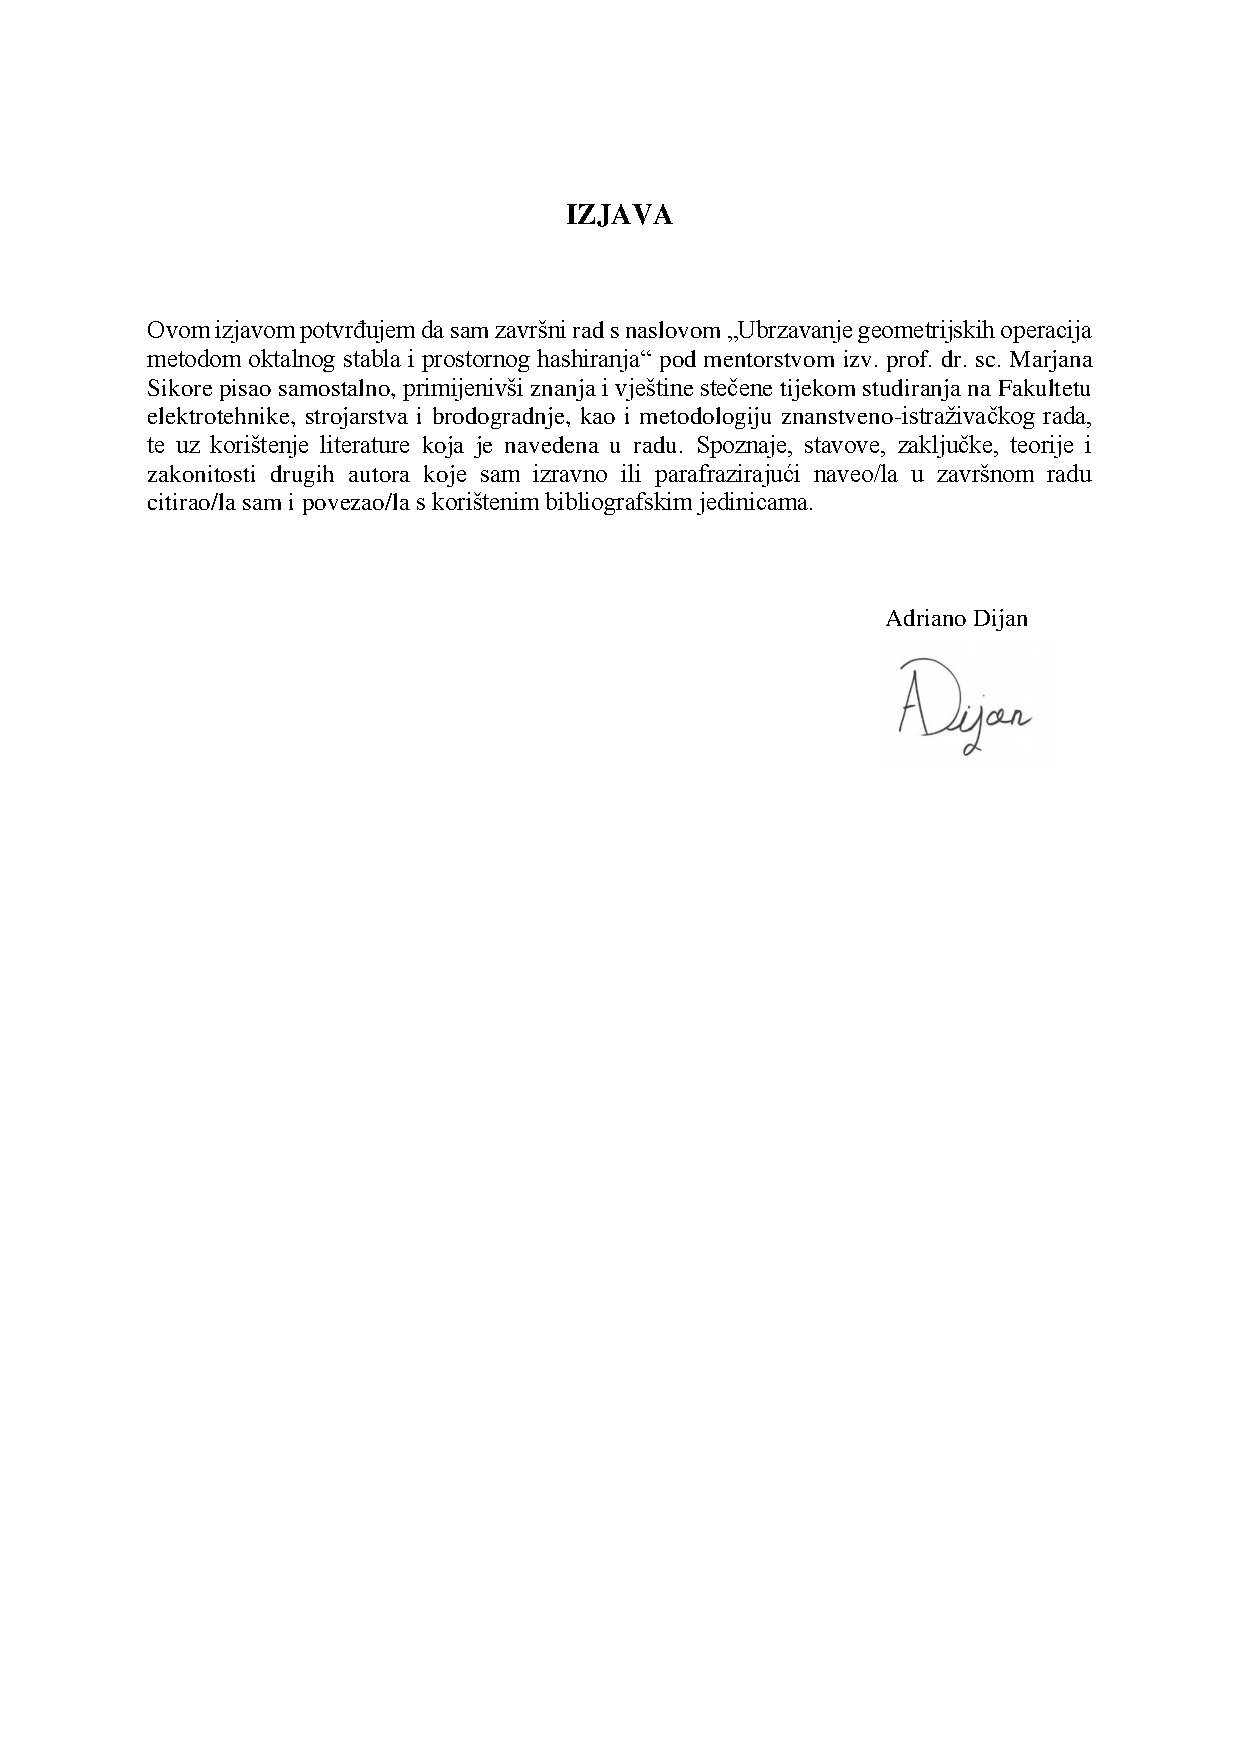
\includepdf[pages=-]{izjava.pdf}
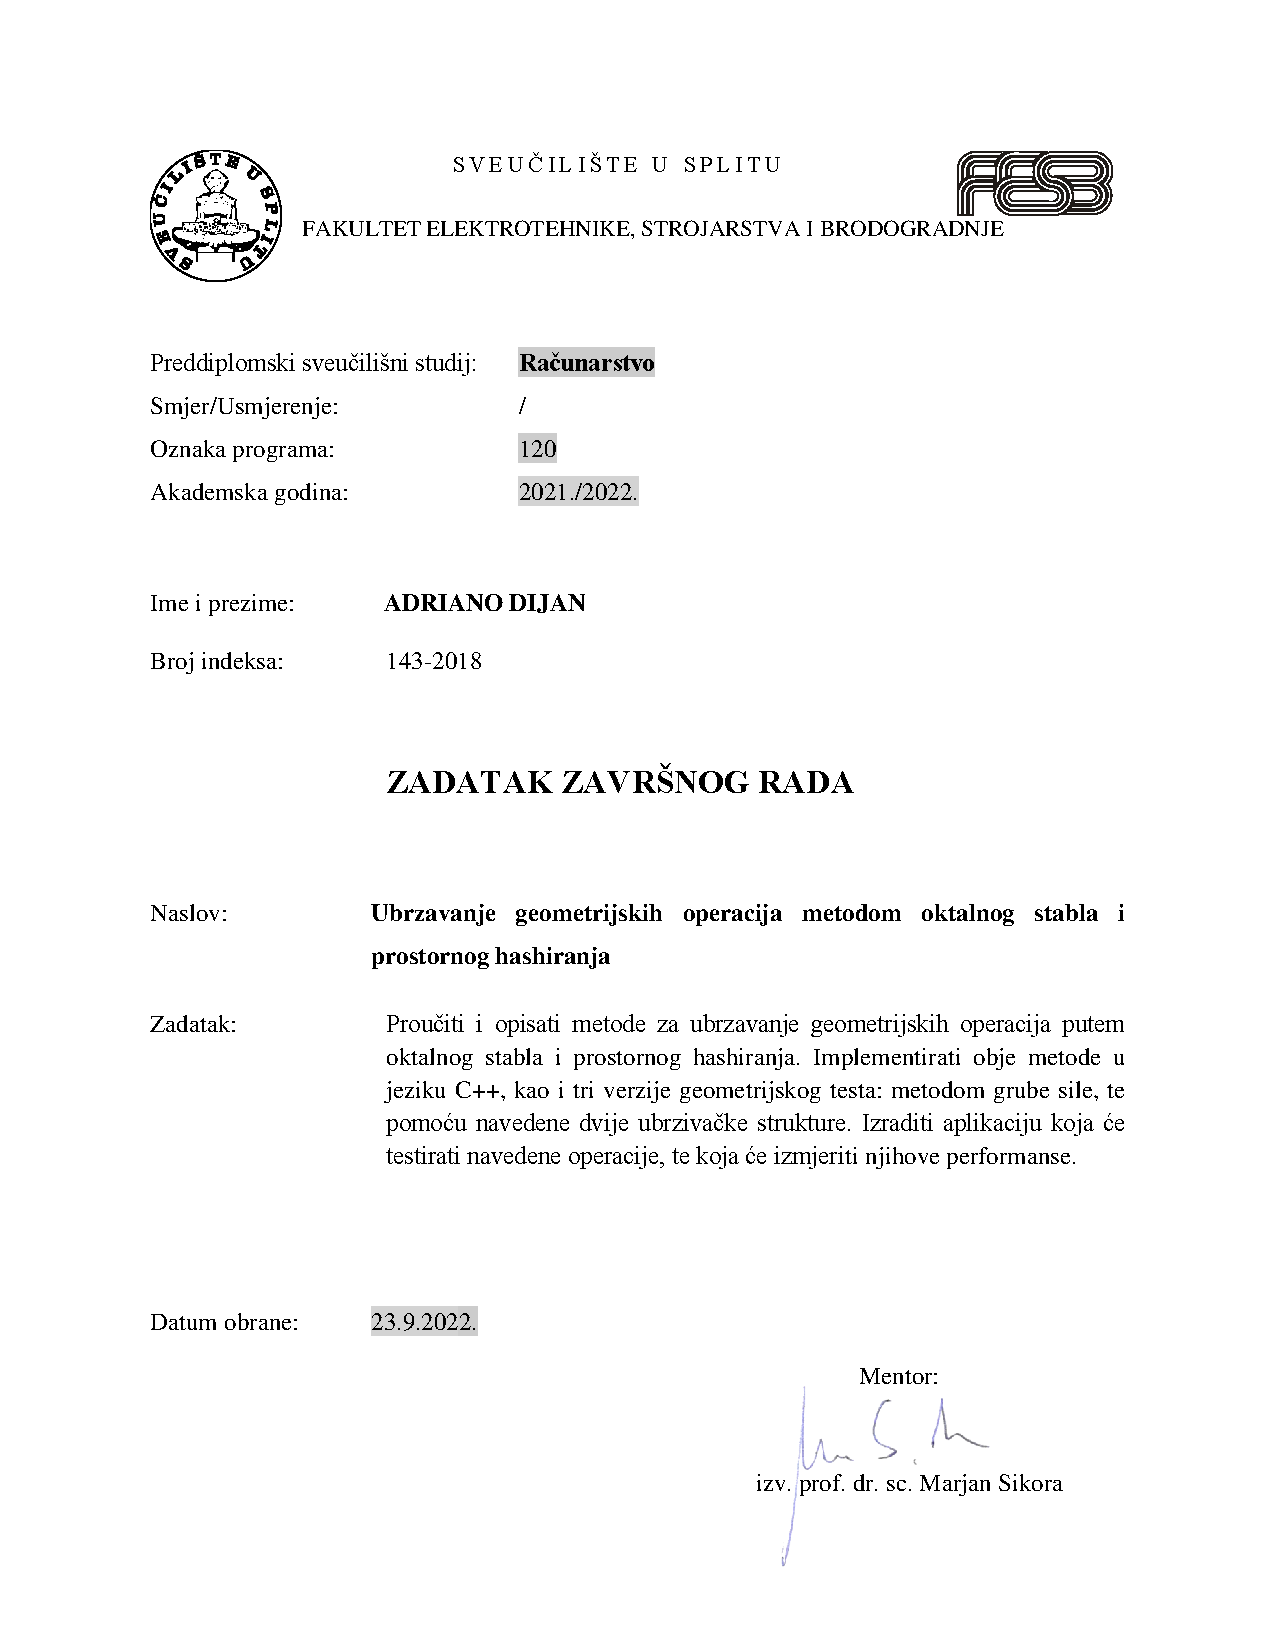
\includepdf[pages=-]{zadatak.pdf}

\newgeometry{top=1cm}
\addtocontents{toc}{\protect\thispagestyle{empty}}
\tableofcontents
\restoregeometry

\pagestyle{plain}
\pagenumbering{arabic}
\chapter{Uvod}

Računalna grafika polje je računarstva koje se bavi digitalnom obradom i prikazom
vizualnih sadržaja korištenjem računala. Jedan od problema koji se često pojavljuje
kod simulacija, videoigara i ostalih područja računalne grafike je otkrivanje sudara
objekata u prostoru.\\
Ovaj rad obradit će tri načina otkrivanja sudara u prostoru, metodu grube sile kao
referentnu vrijednost, te dvije optimizacije, metodu oktalnog stabla i metodu prostornog
hashiranja.\\
Za izradu rada korišten je C++ programski jezik uz Qt biblioteku za izradu grafičkog sučelja
i prikaz modela. Cilj rada je prikazati na koji način i koliko određene metode optimizacije
mogu ubrzati takav tip geometrijskih operacija te usporediti rezultate dobivene na različitim
objektima u prostoru.

\chapter{Alati i tehnologije}

\section{C++}

C++ je programski jezik opće namjene, izvorno napravljen od strane Bjarnea Stroustrupa.
Jezik je nastao kao proširenje programskog jezika C uz dodatak klasa. Moderne verzije jezika C++
podržavaju objektno orijentirano programiranje, generičko programiranje, funkcijski orjetirano programiranje.
Posljednja stabilna verzija standarda ovog programskog jezika je C++20, koji je korišten za izradu ovog rada.~\cite{cpp}

\section{Qt}

Qt je višeplatformsko okruženje za razvoj grafičkih sučelja i višeplatformskih GUI aplikacija.
Omogučava izradu grafičkih sučelja aplikacija za različite platforme uz korištenje standardnog API-ja.
Qt3D, jedna od bibilioteka Qt paketa, pruza mogučnost izrade 3D grafičkih aplikacija. Napisan je u jeziku C++.~\cite{qt}
Pri izradi rada, korišten je za izradu grafičkog sučelja i 3D prikaza objekata nad kojima se izvršava testiranje.

\section{CMake}

CMake je sustav otvorenog koda koji se koristi za automatizaciju izrade paketa, testiranje, prevođenje i instalaciju
softvera. Koristeći posebnu sintaksu (\textit{CMakeLists.txt}) generira konfiguracijske datoteke za druge programske prevoditelje
(MSVC, GCC, LLVM...) i razvojne okoline (Microsoft Visual Studio, Xcode...). Od verzije Qt6, podržani je način izrade Qt aplikacija. ~\cite{cmake}

\pagebreak
\section{Conan}

Conan je upravitelj paketa za C/C++ programske jezike. Omogućava preuzimanje biblioteka sa javno dostupnih repozitorija
i njihovu automatsku integraciju u programski kod. Moguće ga je integrirati sa CMake sustavom kako bi se postiglo automatsko
prevođenje i povezivanje potrebnih biblioteka sa izvornim kodom. Koristeći datoteku \textit{conanfile.py} moguće je definirati
skup pravila po kojima će se biblioteka ili programski paket prevoditi i pakirati, a takav paket je onda moguće koristiti lokalno
ili ga objaviti na javno dostupnom Conan repozitoriju.

\begin{pythonSource}{Primjer konfiguracijske datoteke (\textit{conanfile.py})}
from conans import ConanFile, CMake


class YAAACDConan(ConanFile):
    name = "yaaacd"
    version = "1.0"
    settings = "os", "compiler", "arch", "build_type"
    options = {"shared": [True, False]}
    default_options = "shared=False"
    generators = "cmake"
    exports_sources = (
        "src/*",
        "include/*",
        "CMakeLists.txt",
        "test/*"
    )

        cmake.definitions["CMAKE_BUILD_TYPE"] = str(
            self.settings.build_type
        ).upper()
        cmake.configure()
        return cmake

    def build(self):
        cmake = self._configure_cmake()
        cmake.build()
        cmake.test()

    def package(self):
        cmake = self._configure_cmake()
        cmake.install()

    def package_info(self):
        self.cpp_info.libs = ["yaaacd"]
\end{pythonSource}

\pagebreak

\section{Catch2}

Catch2 je bibilioteka korištena za testiranje C++ koda YAAACD biblioteke.
Omogućava jednostavno pisanje jediničnih testova uz korištenje dostupnih
\textit{macro}-a, automatsku registraciju testova i testove performansi.
Integrira se sa CMake paketom te ga je moguće koristiti sa CTest alatom
za testiranje.

\begin{cppSource}{Primjer Catch2 jediničnog testa}
TEST_CASE("Test octree collision", "[octree]") {
    std::vector<Triangle> triangles;

    std::vector<Vertex> vertices1{
        Vertex(0, 0, 0),
        Vertex(0, 0, 1),
        Vertex(0, 1, 0),
        Vertex(0, 1, 1),
        Vertex(1, 0, 0),
        Vertex(1, 0, 1),
        Vertex(1, 1, 0),
        Vertex(1, 1, 1),
    };

    std::vector<Vertex> vertices2;
    std::transform(
        vertices1.begin(),
        vertices1.end(),
        std::back_inserter(vertices2),
        [](const Vertex& vertex) {
            return Vertex(vertex.x + 0.5, vertex.y + 0.5, vertex.z + 0.5);
        }
    );

    std::vector<Triangle> cube1{
        {vertices1[0], vertices1[6], vertices1[4]},
        {vertices1[0], vertices1[2], vertices1[6]},
        {vertices1[0], vertices1[3], vertices1[2]},
        {vertices1[0], vertices1[1], vertices1[3]},
        {vertices1[2], vertices1[7], vertices1[6]},
        {vertices1[2], vertices1[3], vertices1[7]},
        {vertices1[4], vertices1[6], vertices1[7]},
        {vertices1[4], vertices1[7], vertices1[5]},
        {vertices1[0], vertices1[4], vertices1[5]},
        {vertices1[0], vertices1[5], vertices1[1]},
        {vertices1[1], vertices1[5], vertices1[7]},
        {vertices1[1], vertices1[7], vertices1[3]},
    };

    std::vector<Triangle> cube2{
        {vertices2[0], vertices2[6], vertices2[4]},
        {vertices2[0], vertices2[2], vertices2[6]},
        {vertices2[0], vertices2[3], vertices2[2]},
        {vertices2[0], vertices2[1], vertices2[3]},
        {vertices2[2], vertices2[7], vertices2[6]},
        {vertices2[2], vertices2[3], vertices2[7]},
        {vertices2[4], vertices2[6], vertices2[7]},
        {vertices2[4], vertices2[7], vertices2[5]},
        {vertices2[0], vertices2[4], vertices2[5]},
        {vertices2[0], vertices2[5], vertices2[1]},
        {vertices2[1], vertices2[5], vertices2[7]},
        {vertices2[1], vertices2[7], vertices2[3]},
    };

    Octree tree1(cube1);
    Octree tree2(cube2);

    REQUIRE(tree1.collides(&tree2));
}
\end{cppSource}
\chapter{Oktalno stablo}
\label{chapter:octree}

Oktalno stablo (\textit{Octree}) je struktura podataka kod koje svaki čvor stabla
ima točno 8 čvorova djece. Često se koristi u računalnoj grafici i geometriji,
jer omogućava jednostavnu rekurzivnu podjelu prostora na oktante. Primjenjuje se
u raznim algoritmima optimizacije geometrijskih operacija zbog velike efikasnosti. ~\cite{octree}

\begin{figure}[ht]
    \centering
    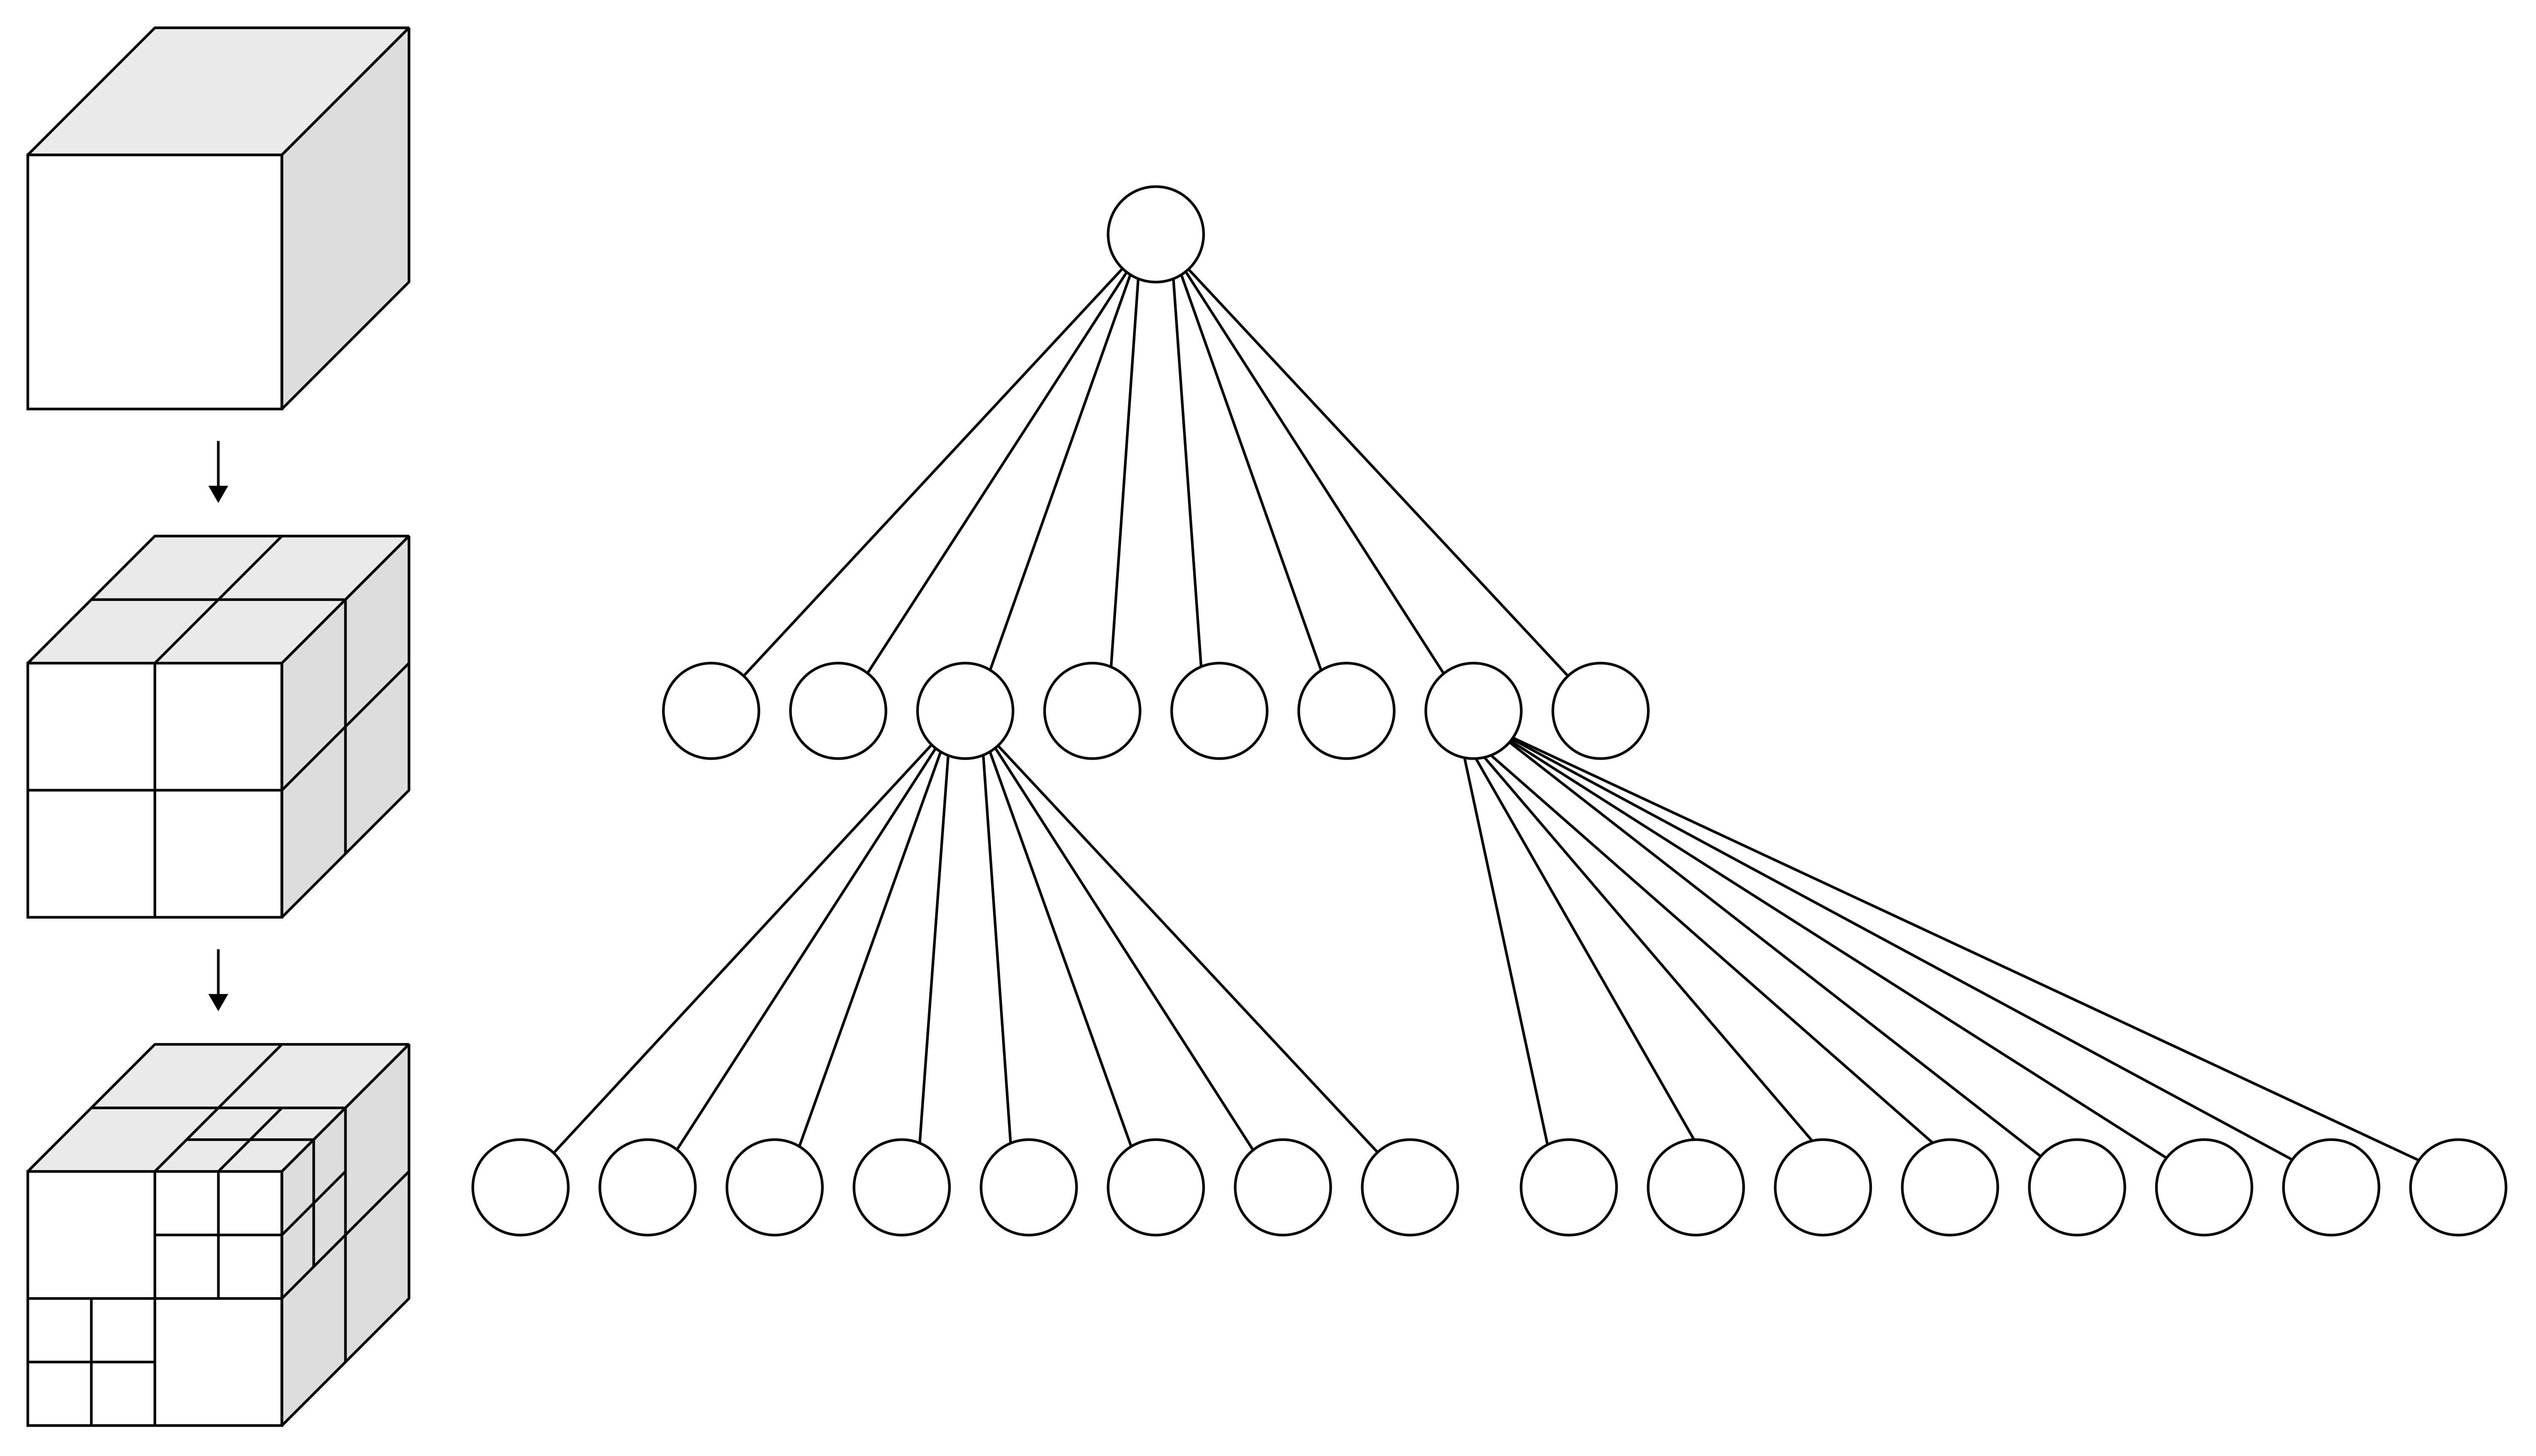
\includegraphics[width=15cm]{octree.png}
    \caption {Prikaz strukture oktalnog stabla}
\end{figure}

\section{Metode grananja}
\subsection{Potpuno oktalno stablo}

Potpuno oktalno stablo je podvrsta oktalnog stabla kod koje svaki unutarnji čvor
ima točno osam čvorova djece. Kod potpunog oktalnog stabla, broj čvorova na najnižoj razini
moguće je odrediti unaprijed kao
\[n_{razina} = 2^{3\cdot razina}\]

Nedostaci potpunog oktalnog stabla su veliko zauzeće memorije, kao i činjenica da će za većinu
modela nepravilnog oblika većina oktanata biti prazna.

\subsection{Grananje po potrebi}

Za razliku od potpunog oktalnog stabla, kod ovakvog tipa strukture čvorovi se granaju ovisno o zadanim
kriterijima, što će ponekad rezultirati neravnomjernom raspodjelom oktanata unutar stabla. Djelovi strukture
koji sadrže više primitivnih objekata granat će se na više razina, dok će oni djelovi koji imaju manje 
takvih objekata biti granani na manje razina.\\
Prednost ovakvog tipa strukture je puno manje zauzeće memorije i puno brža mogućnost pretrage, s obzirom
da velik broj čvorova nije potrebno provjeravati

\section{Primjena kod pronalaženja sudara}

Struktura oktalnog stabla implementirana je u ovom radu kao metoda optimizacije detekcije sudara dvaju trodimenzionalnih objekata.
Objekti nad kojima se vrši detekcija sudara su strukture predstavljene kao mreža trokuta, a učitavaju se iz \textit{Wavefront OBJ} datoteka.
Korišteno je grananje po potrebi (\textit{Branch-on-need}), a broj razina dubine stabla ograničen je na pet.
\pagebreak
\subsection{Parametri oktalnog stabla}

Svaki čvor oktalnog stabla opisan je sa 4 parametra koji su definirani kao članske varijable klase \textit{Octree}

\begin{enumerate}
  \item \textit{members} - svi primitivi (trokuti) koji se (dijelom ili potpuno) nalaze u tom čvoru stabla
  \item \textit{bounds} - objekt tipa \textit{BoundingBox} koji sadržava AABB (Axis-aligned bounding box)
  \item \textit{children} - niz od osam pokazivača na čvorove djecu
  \item \textit{level} - dubina u odnosu na korijenski čvor
\end{enumerate}

Kako bi se pojednostavnila implementacija, svaki od čvorova djece (razine veće od 0) sadrži i pokazivač na korijenski čvor.
\\\\
\textit{BoundingBox} je klasa koja definira strukturu tipa AABB (Axis-aligned bounding box). Koristi se na nultom čvoru za definiranje
kvadra koji opisuje 3D tijelo. Kod čvorova djece rekurzivno se dijeli do definiranih ograničenja, a opisuje prostor koji svaki od 
čvorova oktalnog stabla predstavlja.\\
Definiran je skupom od 8 točaka koji predstavljaju vrhove kvadra, te jednom točkom koja predstavlja njegov centar.
Indeksi vrhova određeni su prema pravilu tablice istinitosti.
\begin{center}
  \begin{tabular}{ c | c | c | c }
    \textbf{INDEX} & \textbf{RIGHT} & \textbf{TOP} & \textbf{FRONT} \\
    \hline
    0 & 0 & 0 & 0 \\
    1 & 0 & 0 & 1 \\
    2 & 0 & 1 & 0 \\
    3 & 0 & 1 & 1 \\
    4 & 1 & 0 & 0 \\
    5 & 1 & 0 & 1 \\
    6 & 1 & 1 & 0 \\
    7 & 1 & 1 & 1
  \end{tabular}
\end{center}

Prema tablici, vrh s indeksom 0 je onaj lijevi, donji i stražnji, a vrh s indeksom 7 - desni, gornji i prednji.
Takav raspored točaka odgovara i rasporedu koordinata u računalnoj grafici. U odnosu na standardni kartezijev
koordinatni sustava, u računalnoj grafici osi \textit{y} i \textit{z} su zamijenjene (Slika \ref{coordinate-system}).


\begin{figure}[ht]
    \centering
    \includegraphics[width=8cm]{3d_coordinate_system.png}
    \caption {Koordinatni sustav korišten u računalnoj grafici}
    \label{coordinate-system}
\end{figure}

\pagebreak
\subsection{Formiranje strukture}

Struktura oktalnog stabla formira se iz mreže trokuta prema sljedećem algoritmu:
\begin{enumerate}
  \item Instancira se korijenski čvor i izračunjaju se granične vrijenosti pripadajućeg AABB-a
  \item Inicijaliziraju se čvorovi djeca, te se za svakog od njih odredi koji trokuti iz korijenskog čvora mu pripadaju.
  \item Za svaki od čvorova djece odredi se \textit{BoundingBox}
  \item 2. i 3. se ponavaljaju sve dok se ne ispuni neki od uvijeta za prestanak
\end{enumerate}

Kod implementacije ovog rada, za inicijalizaciju čvorova djece koristi se optimizacija lijenog učitavanja. Čvorovi djeca se određuju
tek kad se prvi puta pojavi potreba da se pročitaju, a rezultat se zatim sprema u memoriju kako bi bio dostupan kod budućih pristupa.
Takva optimizacija omogućava da se inicijalizacija čvorova djece odgodi tek za vrijeme pristupa (izvršavanje algoritma otkrivanja sudara).
Zbog načina na koji je izveden algoritam otkrivanja sudara, moguće je da (ovisno o međusobnim položajima objekata koji se testiraju)
neke čvorove nikad neće biti potrebno dijeliti na čvorove djecu.

\section{Algoritam otkrivanja sudara}

Algoritam otkrivanja sudara temelji se na činjenici da se dva objekta ne mogu sudarati ako se ne sudaraju \textit{AABB}-ovi koji ih opisuju.


\begin{cppSource}{Implementacija algoritma provjere sudara}
  bool Octree::collides(Octree* octree) {
    std::vector<Octree*> pairs = {this, octree};

    while (!pairs.empty()) {
        Octree* tree1 = pairs.back();
        pairs.pop_back();

        Octree* tree2 = pairs.back();
        pairs.pop_back();

        if (!tree1->bounds().intersects(tree2->bounds())) continue;

        switch (Octree::children_position(tree1, tree2)) {
            case CHILDREN_NONE:
                if (helpers::primes_intersect({tree1->_members, tree2->_members}
                    )) {
                    return true;
                }
                break;
            case CHILDREN_1:
                for (auto child : tree1->children())
                    if (child) {
                        pairs.push_back(child);
                        pairs.push_back(tree2);
                    }
                break;
            case CHILDREN_2:
                for (auto child : tree2->children())
                    if (child) {
                        pairs.push_back(tree1);
                        pairs.push_back(child);
                    }
                break;
            case CHILDREN_BOTH:
                for (auto child1 : tree1->children())
                    for (auto child2 : tree2->children())
                        if (child1 && child2) {
                            pairs.push_back(child1);
                            pairs.push_back(child2);
                        }
                break;
            default:
                break;
        }
    }

    return false;
  }
\end{cppSource}

\pagebreak
Algoritam otkriva sudare na sljedeći način:
\begin{enumerate}
  \item Inicijalizira se stog na kojem se u početku nalaze korijenski čvorovi stabala koja želimo provjeriti
  \item Dok god postoje elementi na stogu, ponavlja se:

  \begin{enumerate}[2.1.]
    \item Skini par čvorova sa stoga
    \item Ako se \textit{AABB}-ovi tog para ne sudaraju, preskoči taj par
    \item Odredi imaju li čvorovi djecu, i koji od njih\\
    Postoje četiri mogućnosti:
    \begin{enumerate}
        \item \textbf{CHILDREN\_NONE} niti jedan od čvorova nema djecu
        \item \textbf{CHILDREN\_1} samo prvi čvor ima djecu
        \item \textbf{CHILDREN\_2} samo drugi čvor ima djecu
        \item \textbf{CHILDREN\_BOTH} oba čvora imaju djecu
    \end{enumerate}
    \item Ako nijedan čvor nema djecu, provjeri sijeku li se primitivi (trokuti) unutar tih čvorova. Ako se trokuti sijeku, algoritam završava s pozitivnim odgovorom.
    \item Ako samo prvi čvor ima djecu, dodaj na stog sve parove drugog čvora i djece prvog čvora.
    \item Ako samo drugi čvor ima djecu, dodaj na stog sve parove prvog čvora i djece drugog čvora.
    \item Ako oba čvora imaju djecu, dodaj na stog sve parove njihove djece.
  \end{enumerate}
  \item Kad na stogu nema više elemenata, algoritam završava negativnim odgovorom
\end{enumerate}
\chapter{Prostorno hashiranje}
\label{chapter:spatial}

Prostorno hashiranje je metoda reprezentiranja trodimenzionalnog prostora u
jednodimenzionalnoj hash tablici. Temelji se na fiksnoj podjeli prostora na
\textit{AABB}-ove i raspodjelu istih tih \textit{AABB}-ova u čelije tablice. ~\cite{gamedev}

\section{Priprema strukture za hashiranje}

Konstruktor hash tablice, kao i konstruktor \textit{Octree} strukture, kao argumente
prima mrežu trokuta od kojih je napravljen trodimenzionalni objekt, kao i željenu
dubinu podjele prostora. Za razliku od oktalnog stabla, kod prostornog hashiranja
ne događa se rekurzivna podjela prostora na oktante, već se prostor podijeli na
fiksni broj \[n = 2^{(3\cdot l)}\] \textit{AABB}-ova, gdje je \textit{l} broj
željenih razina podjele. \\ Na primjer, ako želimo prostor podijeliti 5 puta,
broj \textit{AABB}-ova bit će 32768.

\begin{cppSource}{Implementacija funkcije za podjelu prostora}
std::vector<BoundingBox *>
BoundingBox::split(int level, const std::vector<Triangle> &triangles) {
    std::deque<BoundingBox *> queue;
    auto this_children = this->children();
    std::for_each(
        this_children.begin(),
        this_children.end(),
        [&queue, &triangles](BoundingBox *child) {
            queue.push_back(child);
            std::copy_if(
                triangles.begin(),
                triangles.end(),
                std::back_inserter(child->members()),
                [&child](const Triangle &triangle) {
                    return child->contains(triangle);
                }
            );
        }
    );

    while (queue.front()->level() != level) {
        std::array<BoundingBox *, 8> box_children = queue.front()->children();
        std::for_each(
            box_children.begin(),
            box_children.end(),
            [&queue](BoundingBox *child) {
                queue.push_back(child);
                std::copy_if(
                    queue.front()->members().begin(),
                    queue.front()->members().end(),
                    std::back_inserter(child->members()),
                    [&child](const Triangle &triangle) {
                        return child->contains(triangle);
                    }
                );
            }
        );
        queue.pop_front();
    }

    std::vector<BoundingBox *> retval(std::begin(queue), std::end(queue));

    return retval;
}
\end{cppSource}

\pagebreak
\section{Hash funkcija}

Hash funkcija koja se koristi kod prostornog hashiranja definirana je kao

\begin{equation}
    h = (\lfloor \frac{x}{k} \cdot P_1 \rfloor \oplus \lfloor \frac{y}{k} \cdot P_2 \rfloor \oplus \lfloor \frac{z}{k} \cdot P_2 \rfloor) \mod t
\end{equation}

gdje je \textit{t} veličina hash tablice, \textit{k} predefinirana
konstantna vrijednost, a $ P_{1..3} $ proizvoljno velik prost broj. ~\cite{spatialhashing}

\begin{cppSource}{Implementacija hash funkcije u jeziku C++}
int SpatialHashMap::_hash(BoundingBox* box) {
    Vertex center = box->center();

    return (static_cast<int>(center.x / CELL_SIZE * P1) ^
            static_cast<int>(center.y / CELL_SIZE * P2) ^
            static_cast<int>(center.z / CELL_SIZE * P3)) %
           TABLE_SIZE;
}
\end{cppSource}

\section{Stvaranje hash tablice}

Umetanje točaka u hash tablicu odvija se prema sljedećem algoritmu:

\begin{enumerate}
    \item Izračuna se hash vrijednost točke
    \item Ako u hash tablici već postoji ta vrijednost, točka se dodaje u \textit{vector}
    \item Ako vrijednost ne postoji, stvori se novi ključ te se inicijalizira \textit{vector}
          u kojeg se umetne ta točka
\end{enumerate}

Zbog jednostavnosti algoritma i optimizacije performansi, hash funkcija se ne
računa za svaki trokut mreže, već se \textit{hashiraju} samo središnje točke
\textit{AABB}-ova. Nakon što je poznata hash vrijednost središnje točke, u
hash tablicu se umeću svi trokuti koji pripadaju tom \textit{AABB}-u.


\begin{cppSource}{Umetanje \textit{AABB}-ova u hash tablicu}
void SpatialHashMap::insert(BoundingBox* box) {
    int hash = this->_hash(box);

    if (!box->members().size()) return;

    std::map<int, std::vector<Triangle>>::iterator cell = this->_map.find(hash);
    if (cell != this->_map.end()) {
        std::copy(
            box->members().begin(),
            box->members().end(),
            std::back_inserter(cell->second)
        );
        return;
    }

    this->_map.insert_or_assign(hash, box->members());
}
\end{cppSource}

\section{Algoritam za otkrivanje sudara}

Algoritam za otkrivanje sudara korištenjem hash
tablice izveden je sljedećim algoritmom:

\begin{enumerate}
    \item Objekt s kojim se želi provjeriti sudar podijeli se na jednak broj razina kao i 
          postojeći objekt u hash tablici
    \item Za svaki od \textit{AABB}-ova:
    \begin{enumerate}[i.]
        \item Izračuna se hash vrijednost
        \item Ako ta vrijednost postoji u hash tablici, provjeravaju
              se svi trokuti iz te čelije tablice
        \item Ako ta vrijednost ne postoji u tablici, prelazi se na sljedeći čvor
    \end{enumerate}
\end{enumerate}

\begin{cppSource}{Algoritam za otkrivanje sudara}
bool SpatialHashMap::collides(const std::vector<Triangle>& triangles) {
    std::vector<Vertex> vertices;

    for (const Triangle& triangle : triangles)
        std::for_each(
            triangle.begin(),
            triangle.end(),
            [&vertices](const Vertex& vertex) {
                vertices.push_back(vertex);
            }
        );

    BoundingBox root(vertices);
    std::vector<BoundingBox*> children = root.split(this->_levels, triangles);

    return std::any_of(children.begin(), children.end(), [&](BoundingBox* box) {
        int hash = this->_hash(box);

        auto cell = this->_map.find(hash);
        if (cell != this->_map.end()) {
            return helpers::primes_intersect({cell->second, box->members()});
        }

        return false;
    });
}
\end{cppSource}
\chapter{Testiranje performansi}

Biblioteka YAAACD izrađena je u svrhu usporedbe performansi triju vrsti
algoritama otkrivanja sudara u trodimenzionalnom prostoru.

Upoređivani algoritmi su:
\begin{enumerate}
    \item \textbf{Algoritam grube sile} - vrsta provjere u kojoj se
          provjeravaju svi primitivi dvaju učitanih objekata
    \item \textbf{Provjera korištenjem oktalnog stabla} - opisano u poglavlju \ref{chapter:octree}
    \item \textbf{Provjera korištenjem prostornog hashiranja} - opisano u poglavlju \ref{chapter:spatial}
\end{enumerate}

\section{Način testiranja}

Testiranje je izvedeno korištenjem YAAACD-GUI aplikacije, koja se brine za grafički prikaz
objekata koji se testiraju, mjerenje performansi te izvještavanje (\textit{logging}) (Slika \ref{logging}).

\begin{figure}[h!]
    \centering
    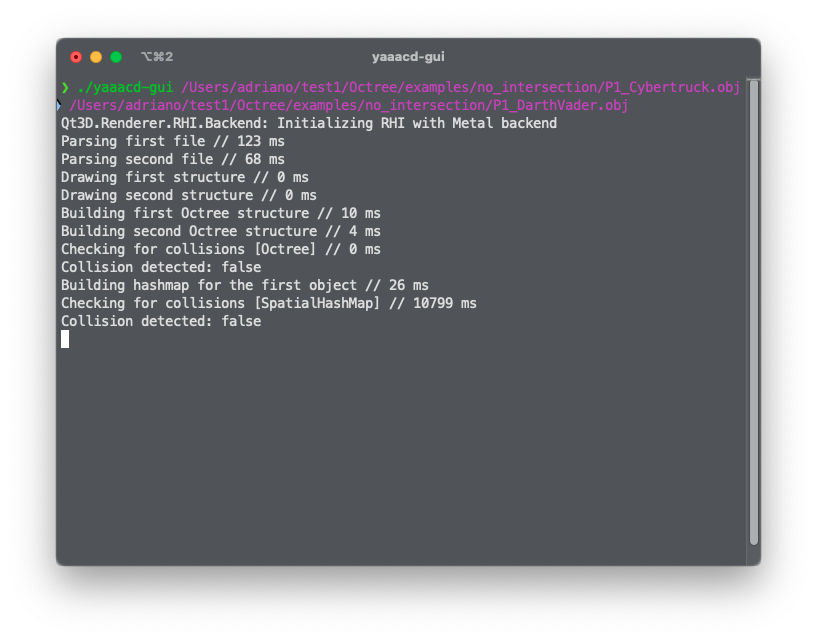
\includegraphics[width=12cm]{logs.png}
    \caption {Prikaz ispisa aplikacije YAAACD-GUI prije učitavanja.}
    \label{logging}
\end{figure}

\pagebreak
\subsection{Testno okruženje}
Sve metode korištenje pri testiranju koriste samo jednu procesorsku nit.
Testiranje je izvršeno na sustavu sa Intel Core i7 procesorom, 16 GB radne memorije
i macOS operacijskim sustavom. (Slika \ref{testbench})

\begin{figure}[h!]
    \centering
    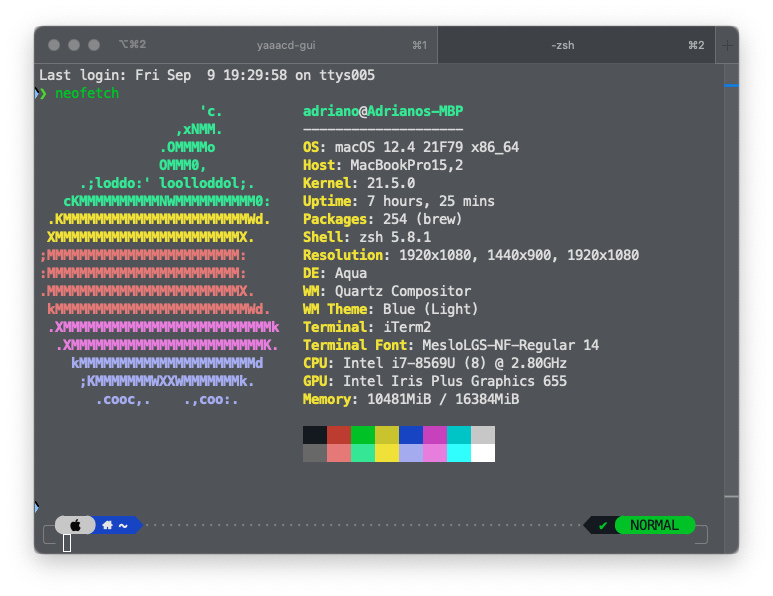
\includegraphics[width=12cm]{testbench.png}
    \caption {Prikaz informacija o testnom sustavu}
    \label{testbench}
\end{figure}

\pagebreak
\section{Rezultati testiranja}

Testiranje je izvedeno sa četiri različita 3D modela različite veličine i gustoće primitiva.
Rezultati su prikazani u tablici \ref{table:testresults}

\begin{table}[h!]
    \begin{center}
      \begin{tabular}{ | c | c | c | }
        \hline
        \textbf{Model} & \textbf{Broj točaka} & \textbf{Broj trokuta} \\
        \hline
         Spiderman (Slika \ref{model:spiderman}) & 74.999 & 149.994 \\
        \hline
         Cybertruck (Slika \ref{model:cybertruck}) & 32.273 & 63.614 \\
        \hline
         Shrek (Slika \ref{model:shrek}) & 1.274 & 2.332 \\
        \hline
         Darth Vader (Slika \ref{model:darthvader}) & 24.636 & 35.624 \\
        \hline
      \end{tabular}
    \end{center}
  \caption{Broj poligona i točaka po modelu}
  \label{table:poly}
\end{table}

\begin{figure}
    \centering
    \begin{minipage}[b]{0.4\textwidth}
        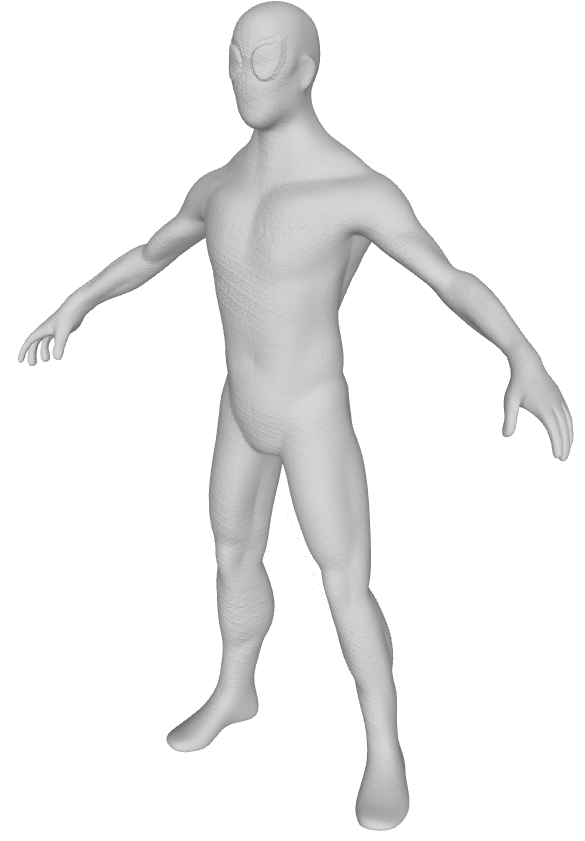
\includegraphics[width=\textwidth]{spiderman.png}
        \caption {Testni model: Spiderman}
        \label{model:spiderman}
    \end{minipage}
    \begin{minipage}[b]{0.4\textwidth}
        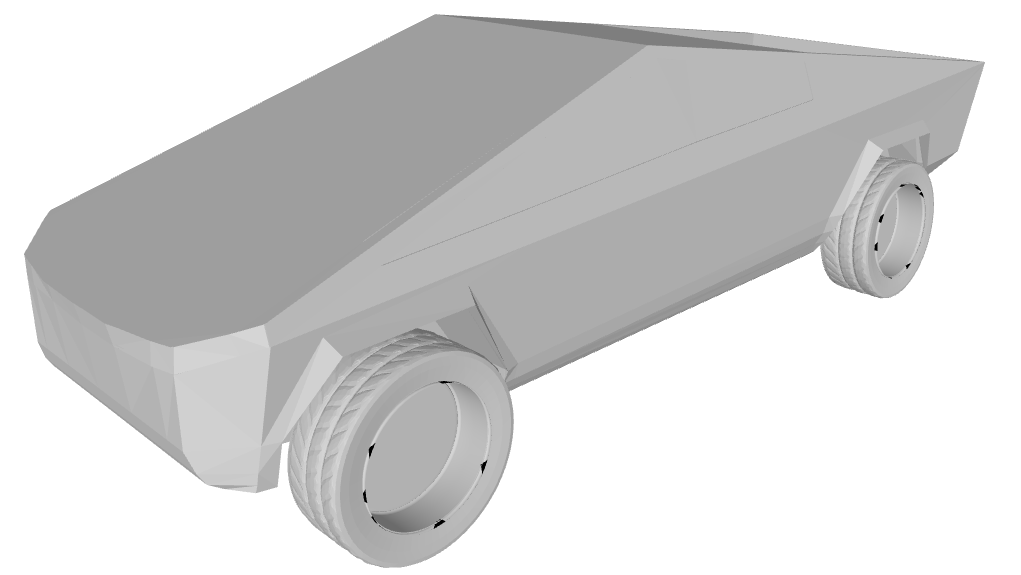
\includegraphics[width=\textwidth]{cybertruck.png}
        \caption {Testni model: Cybertruck}
        \label{model:cybertruck}
    \end{minipage}
    \begin{minipage}[b]{0.4\textwidth}
        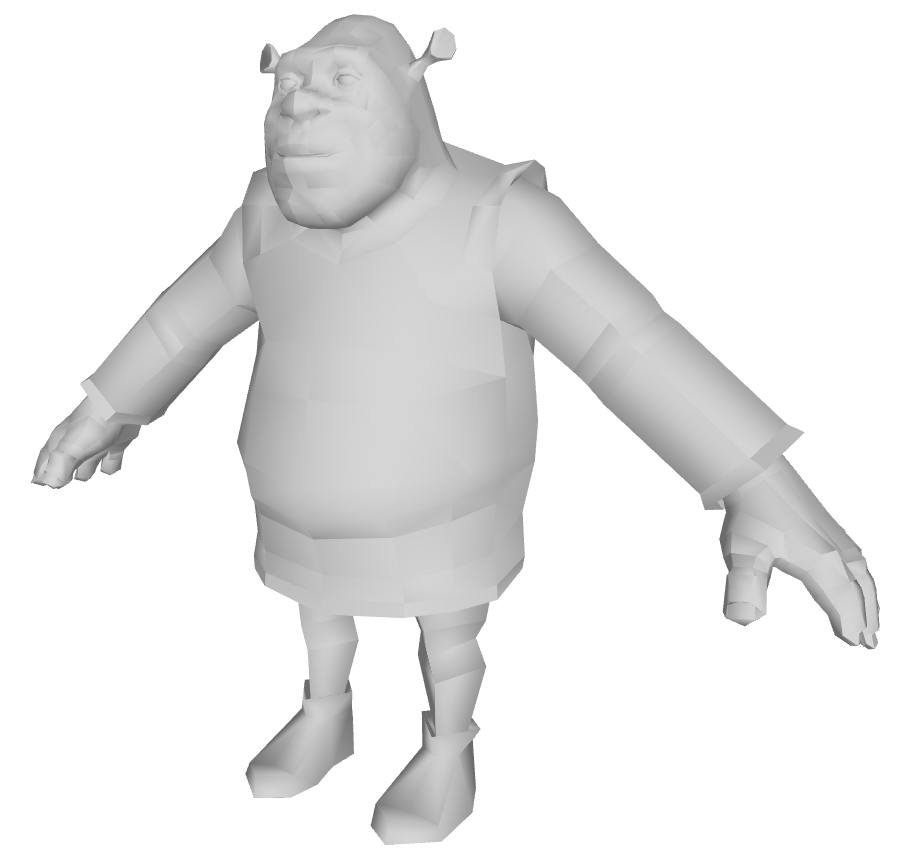
\includegraphics[width=\textwidth]{shrek.png}
        \caption {Testni model: Shrek}
        \label{model:shrek}
    \end{minipage}
    \begin{minipage}[b]{0.4\textwidth}
        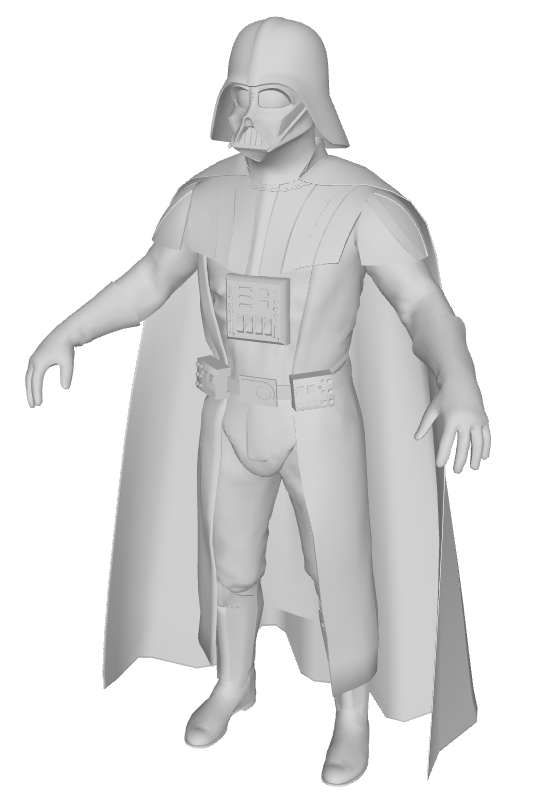
\includegraphics[width=\textwidth]{darthvader.png}
        \caption {Testni model: Darth Vader}
        \label{model:darthvader}
    \end{minipage}
\end{figure}

\begin{table}[h!]
    \begin{center}
      \begin{tabular}{ | c | c | c | c | }
        \hline
        \textbf{Modeli} & \textbf{Odnos objekata} & \textbf{Algoritam} & \textbf{Trajanje (ms)} \\
        \hline
         Cybertruck / Darth Vader & Sijeku se & Oktalno stablo & 68 \\
        \hline
         Cybertruck / Darth Vader & Sijeku se & Prostorno hashiranje & 82 \\
        \hline
         Cybertruck / Darth Vader & Sijeku se & Bruteforce & 643 \\
        \hline
         Shrek / Spiderman & Sijeku se & Oktalno stablo & 78 \\
        \hline
         Shrek / Spiderman & Sijeku se & Prostorno hashiranje & 517 \\
        \hline
         Shrek / Spiderman & Sijeku se & Bruteforce & 27839 \\
        \hline

         Cybertruck / Darth Vader & Ne sijeku se & Oktalno stablo & $<$1 \\
        \hline
         Cybertruck / Darth Vader & Ne sijeku se & Prostorno hashiranje & 10736 \\
        \hline
         Cybertruck / Darth Vader & Ne sijeku se & Bruteforce & 393867 \\
        \hline
         Shrek / Spiderman & Ne sijeku se & Oktalno stablo & $<$1 \\
        \hline
         Shrek / Spiderman & Ne sijeku se & Prostorno hashiranje & 685 \\
        \hline
         Shrek / Spiderman & Ne sijeku se & Bruteforce & 61512 \\
        \hline

         Cybertruck / Darth Vader & Sijeku se AABB-ovi & Oktalno stablo & 135 \\
        \hline
         Cybertruck / Darth Vader & Sijeku se AABB-ovi & Prostorno hashiranje & 4942 \\
        \hline
         Cybertruck / Darth Vader & Sijeku se AABB-ovi & Bruteforce & 394121 \\
        \hline
         Shrek / Spiderman & Sijeku se AABB-ovi & Oktalno stablo & 49 \\
        \hline
         Shrek / Spiderman & Sijeku se AABB-ovi & Prostorno hashiranje & 735 \\
        \hline
         Shrek / Spiderman & Sijeku se AABB-ovi & Bruteforce & 61512 \\
        \hline
      \end{tabular}
    \end{center}
  \caption{Rezultati testiranja}
  \label{table:testresults}
\end{table}

\chapter{Grafičko sučelje}

Aplikacija za testiranje realizirana je kao \textit{desktop} aplikacija,
korištenjem Qt i Qt3D biblioteka. Glavni prozor aplikacije sastoji se od 
3D prikaza u kojem je moguće vidjeti modele koji su trenutno učitani, a
u donjem dijelu glavnog prozora vidljiv je prozor informacija \textit{log box}
u kojem je moguće vidjeti izmjerene performanse. (Slika \ref{gui})

Aplikacija se pokreće tako da se izvršna datoteka pozove s 2 argumenta koji moraju
biti putanje do dviju \textit{.obj} datoteka. Moguće je proslijediti i dodatni argument
(\textit{--bruteforce}), kojim će se pokrenuti i testiranje metodom grube sile.

\begin{figure}[h!]
    \centering
    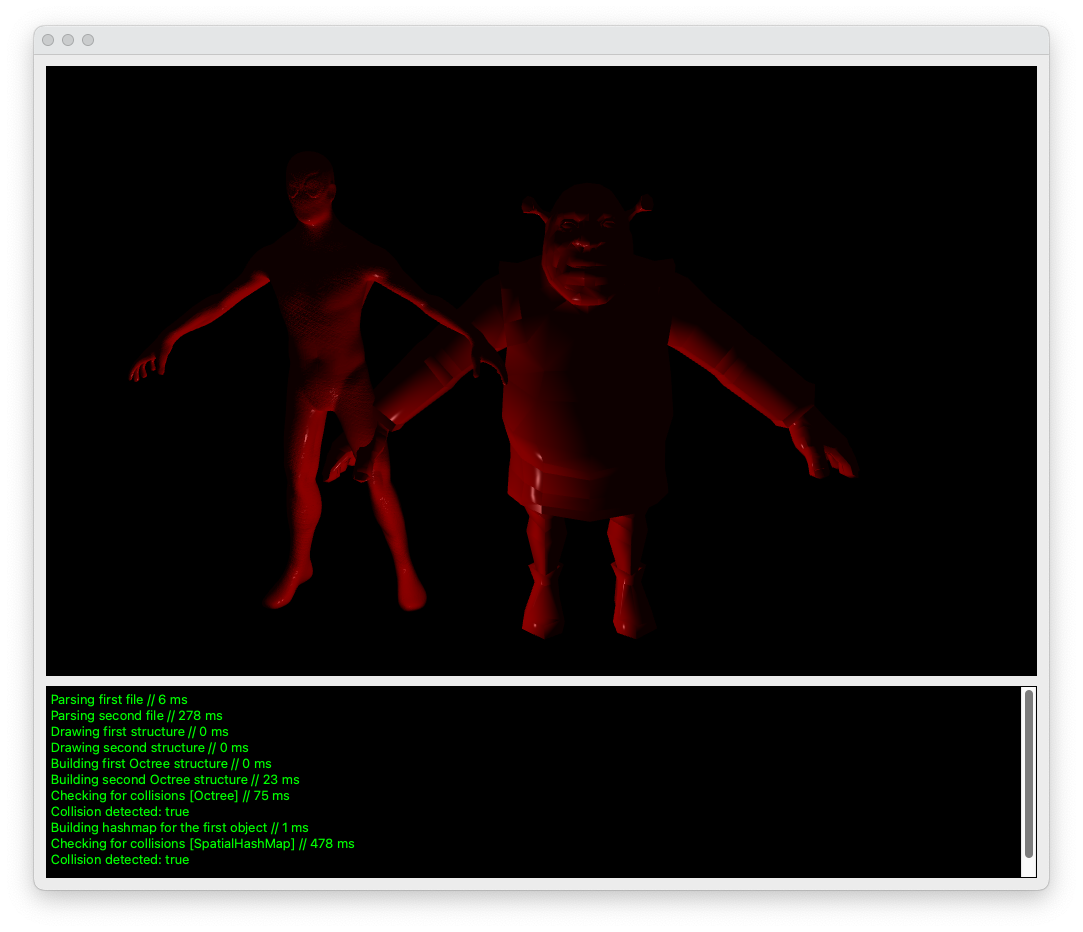
\includegraphics[width=12cm]{gui.png}
    \caption {Izgled glavnog prozora aplikacije}
    \label{gui}
\end{figure}

Trajanje svakog koraka algoritma izmjereno je korištenjem \textit{chrono} biblioteke
Nakon što se algoritam izvrši, modele je moguće vidjeti u glavnom prozoru, a rezultate
testiranja u donjem prozoru za informacije.

\begin{cppSource}{Implementacija funkcije za grafički prikaz modela}
void View3D::add_obj_file(std::string filename) {
    Qt3DCore::QEntity *mesh_entity = new Qt3DCore::QEntity(this->root_entity);
    Qt3DRender::QMesh *mesh = new Qt3DRender::QMesh(this->root_entity);
    mesh->setSource(QUrl::fromLocalFile(filename.c_str()));

    mesh_entity->addComponent(mesh);
    mesh_entity->addComponent(this->phong_red);
}
\end{cppSource}

\begin{cppSource}{Dio koda za mjerenje trajanja funkcije}
...
start_time = chrono::high_resolution_clock::now();
*(log_box) << "Checking for collisions [Octree] // ";
bool octree_collides = tree1.collides(&tree2);
int duration = chrono::duration_cast<chrono::milliseconds>(
    chrono::high_resolution_clock::now() - start_time
).count();
*(log_box) << duration << " ms\n";
*(log_box) << "Collision detected: "
           << (octree_collides ? "true" : "false") << "\n";
...
\end{cppSource}

\chapter{Zaključak}

Pomoću programske biblioteke i grafičkog programa, ovaj rad prikazuje
način implementacije i usporedbu triju algoritama za otkrivanje sudara
u trodimenzionalnom prostoru.
\\
Prvi dio rada opisuje tehnologije korištene
za realizaciju programske podrške, drugi dio prikazuje algoritme i optimizacije
koje su upotrebljavane, te je na kraju prikazana njihova primjena i rezultati.
\\
Iz rezultata testiranja vidljiv je značajan utjecaj oba algoritma optimizacije
u odnosu na referentni test metodom grube sile. Obje metode pokazale su poboljšanje
performansi do nekoliko redova veličine. Vidljivo je da metoda oktalnog stabla
u nekim slučajevima omogućava otkrivanje sudara objekata nakon samo jedne provjere,
dok je i u slučajevima kad sudar postoji do 1000 puta brža od metode grube sile.
\\
Kod metode prostornog hashiranja, iako u manjoj mjeri, također su vidljiva
značajna poboljšanja performansi. Kako prostorno hashiranje ovisi o većem broju
parametara (veličina čelije, hash funkcija), moguće je kako bi optimizacijom
tih parametara rezultati bili bolji.

\printbibliography[heading=bibintoc, title=Literatura]
\chapter*{Sažetak}
\addcontentsline{toc}{chapter}{Sažetak}

\section*{Sažetak}

Rad se bavi analizom dvaju algoritama optimizacije geometrijskih operacija,
metodom oktalnog stabla i prostornog hashiranja. U radu je prikazana
izrada C++ biblioteke za optimizaciju geometrijskih operacija i izrada
grafičke aplikacije za testiranje bibilioteke. Nakon uvoda u rad,
drugo poglavlje daje pregled korištenih tehnologija i načine na koje
su te tehnologije primjenjene u ovom radu. Sljedeća dva poglavlja
daju opis metoda optimizacije koje su korištene. Peto poglavlje prikazuje
načine i rezultate testiranja, te njihovu analizu. U šestom, posljednjem
poglavlju prije zaključka rada, prikazan je izgled i način funkcioniranja
grafičke aplikacije.

\section*{Ključne riječi}
\textit{
    Oktalno stablo, Prostorno hashiranje, Otkrivanje sudara, Qt3D
}


\chapter*{Summary}
\addcontentsline{toc}{chapter}{Summary}

\textbf{Title: } Optimization of geometric operations using the octal tree method and spatial hashing
\section*{Summary}

This thesis analyzes two algorithms used to optimize geometric operations,
the octal tree method, and the spatial hashing. The thesis demonstrated the process
of creating a C++ library used for the optimization of the geometric operations, 
and the GUI application used for testing the library. Following the introduction,
the second chapter gives a brief overview of the technologies and tools that were used
and the ways that those technologies were applied to this project.
The following two chapters describe the used optimization methods.
The fifth chapter shows the testing methods and provides the testing results
along with the analysis of those. The sixth chapter, the last one before the thesis
conclusion, shows the GUI application and explains the way it works.

\section*{Keywords}
\textit{
    Octree, Spatial hashing, Collision detection, Qt3D
}

\end{document}
